\chapter{Desarrollo}

En el presente capítulo se describirán los pasos y procedimientos realizados para cumplir con los objetivos propuestos para la pasantía y se encuentra dividido en 5 secciones. Cada una representa mejoras incrementales que enriquecieron tanto los aspectos de arquitectura de software como conceptos asociados a las \pwas. Así mismo, cada etapa fue realizada de forma exploratoria, utilizando herramientas y enfoques de desarrollo retroalimentados por los resultados parciales que eran obtenidos.

\section{Migración a Angular 2}

La aplicación web cliente de \business, fue desarrollada inicialmente con el \textit{framework} web de desarrollo AngularJS, en su versión 1. Esta herramienta permitió al equipo de desarrollo desplegar funcionalidades de forma rápida y basada en prototipos. Sin embargo, a medida que el número de requisitos que debe cumplir la aplicación aumenta, y consecuentemente la complejidad de la misma, se requiere hacer uso de herramientas que permitan la escalabilidad del desarrollo con el uso de tecnologías en el estado del arte que permitan la mantenibilidad y extensión del software a mayor escala.

Desde la comunidad de código libre, y con el soporte de Google para su desarrollo, se creó la versión 2 del \textit{framework} `Angular', compartiendo conceptos con su versión anterior pero con la capacidad de atacar muchas más aristas del desarrollo web. Para el momento del desarrollo de la pasantía, aún se encontraba en estado de pre-producción, pero prometiendo ser una herramienta excelente para cumplir con los requisitos de escalabilidad \cite{angularchangelog}.

Durante esta primera etapa, el equipo de Desarrollo, bajo la coordinación del pasante, enfocó buena parte de sus recursos en actualizar la aplicación existente bajo la nueva herramienta. Este proceso se realizó de forma incremental: `Angular 2' tuvo herramientas asociadas que permitían entrelazar componentes de ambas versiones, de manera que nuevas funcionalidades eran agregadas bajo la versión 2, y paulatinamente se fueron migrando componentes pre-existentes de la versión 1 \cite{angularupgrade}. Luego de integrar el uso de ambas herramientas en la plataforma y ajustarlo al sistema de construcción de la aplicación (\textit{builds}), esto permitió seguir manteniendo un ritmo de lanzamiento de funcionalidades aceptable mientras el proceso de actualización era realizado paralelamente. De la misma forma, todo el equipo de desarrollo tuvo la oportunidad de familiarizarse con el nuevo \textit{framework} al implementar o migrar funcionalidades en la plataforma.

\section{Capa de Comunicaciones}

Una de las áreas de la arquitectura de software de la aplicación que mayor atención y diseño se le debía prestar, es al conjunto de servicios y abstracciones relacionado a la comunicación con lo diferentes servidores web. Si bien uno de los objetivos principales de la pasantía consiste en la resiliencia a la conexiones restringidas, las abstracciones deben estar preparadas para manejar de forma flexible estos escenarios, así como cumplir con los requisitos de producto y de desarrollo para una mantenibilidad y facilidad de mejoramiento aceptable.

Entre algunos requisitos de alto nivel que pudieron detectarse al momento de análisis y diseño, se encuentran:

\begin{itemize}
  \item Uso de abstracciones genéricas, adaptables a diferentes orígenes de datos (tanto locales como provenientes de internet).
  \item Disponibilidad de mecanismos para respuesta ante fallas de origen
  \item Flexibilidad y capacidad de personalización para los casos de uso ya existentes en el software
  \item Interoperable con otros componentes del software, así como con otras abstracciones y herramientas asociadas
\end{itemize}

Una implementación basada en el modelo de observables se ajustó correctamente a estos requerimientos: modela eventos que son independientes del origen (eventos del explorador web, respuestas de base de datos o de componentes locales); es firmemente utilizada en el framework Angular, lo cual permite su interoperabilidad; es una librería independiente y reutilizable, flexible a los usos requeridos; y posee un conjunto de herramientas asociados para un fácil desarrollo, así como una comunidad de desarrollo de tamaño considerable. Al analizar que se ajustaba a los requisitos se decidió por experimentar con esta idea en la implementación de un pequeño sistema de carga de imágenes en la aplicación.

Se tuvo como requisito funcional la subida de imágenes de perfil a la aplicación. El usuario debía poder entrar a su perfil y subir una imagen desde su dispositivo y utilizarla como su imagen de su usuario en la plataforma. Además de la carga usual del archivo de la imagen, se requería conocer el progreso de la subida del archivo así como la capacidad de cancelar la subida, y ofrecer al usuario una experiencia de usuario práctica y fácil de usar. Se realizó una implementación en base al modelo de observables que permitió desarrollar la funcionalidad en corto tiempo y con fácil entendimiento de su funcionamiento interno y externo.

Dada la utilidad del modelo, se procedió a usarlo como pilar principal de la capa de comunicación de la aplicación. Aunque el framework Angular provee una serie de herramientas que ya facilitaba la comunicación con servidores usando observables, estas herramientas debían adaptarse a los requisitos particulares establecidos, tanto en manejo de URLs, manejo de datos y otros estándares utilizados de comunicación.

Se decidió realizar una implementación experimental de una meta librería que permitiese personalizarla y ajustarla a los requisitos particulares de la aplicación, sin perder generalidad. Se desarrolló entonces la librería \texttt{reactive-rest} que tiene sólo 2 suposiciones fuertes:

\begin{itemize}
  \item Su uso está orientado a la comunicación con servicios web de tipo RESTful
  \item Su interfaz de programación (API) está basado en observables
\end{itemize}

La implementación de la librería es bastante sencilla y funciona más como un coordinador de componentes que como una ejecución de una lógica específica: provee un esqueleto de firmas externa y entrelaza el flujo de comunicación entre componentes que son personalizables y deben ser provistos por el usuario. La librería no provee estos componentes, sino que provee los espacios (utilizables de formas sencillas) para que el usuario la ajuste a su conveniencia y requerimientos: método de comunicación subyacente, manejo de urls, pre-procesamiento de solicitudes y post-procesamiento de respuestas.

Dada la naturaleza abierta y genérica de esta librería, se liberó como proyecto de código libre en \textit{GitHub} \cite{reactiverestgithub} y la plataforma de distribución \textit{npm} \cite{reactiverestnpm}. La implementación de los componentes particulares es parte del código interno de la plataforma, algunos con el uso de librerías de Angular.

Finalmente, usando la librería \texttt{reactive-rest}, se reimplementó progresivamente la capa de comunicación de la aplicación, bajo el modelo de observables, con lo cual pueden crearse flujos muy flexibles de datos, en particular aquellos necesarios para aplicaciones offline.

\section{Construcción y Distribución}

La siguiente importante meta en los objetivos de la pasantía consistía en mejorar los sistemas de construcción y flujos de distribución de la aplicación, para mejorar su rendimiento y disponibilidad. Uno de los aspectos motivantes al uso y desarrollo de las aplicaciones nativas es la experiencia fluida al accederlas y utilizarlas. En el caso de las aplicaciones web, estos sistemas de construcción y distribución influyen de manera importante en la carga inicial de las mismas en un explorador web. Sistemas de construcción se refiere a los mecanismos y procesos para obtener una aplicación web utilizable a partir del código fuente. Sistemas de distribución se refiere a los sistemas y plataformas establecidos para que un explorador web obtenga la aplicación previamente construida.

En el sistema pre-existente, la construcción de la aplicación era basada en las herramientas \textit{systemjs} y \textit{gulp}, desarrollado con cierto nivel de personalización. La distribución de la aplicación era basada en un servidor web en el \textit{runtime nodejs}, personalizado ligeramente. Una reestructuración de estos sistemas debía permitir facilitar la capacidad de agregar nuevas funcionalidades de forma escalable (tanto en desarrollo como tráfico de usuarios), simplificar la mantenibilidad de los sistemas y utilizar las mejores prácticas del estado del arte. En particular, debían tomarse a consideración la implementación o utilización de los mecanismos orientados al uso de los diferentes tipos de caché disponibles y otros ajustes que puedan acelerar la carga inicial de la aplicación.

Para el sistema de construcción se decidió cambiar los elementos principales implementados manualmente con \textit{gulp} por el uso de la herramienta `Angular CLI' \cite{angularcli}. Esta herramienta simplifica el sistema de construcción y su mantenibilidad, dado que la implementación existe de forma externa al proyecto principal, y es mantenida por Google y la comunidad de código libre. Igualmente, provee una mayor profundidad en algunos aspectos de la construcción. Aquellos aspectos que no son cubiertos por la herramienta, siguen implementados con \textit{gulp}.

Algunas de las funcionalidades clave, motivantes a su uso, que posee la herramienta con respecto a la velocidad:

\begin{itemize}
  \item \textit{Bundling}: la aplicación es compactada en un pequeño número de archivos, para reducir el número de solicitudes realizadas por el explorador web y optimizar la carga inicial.
  \item \textit{Hashing}: los archivos generados son nombrados de forma única dependiendo de sus contenidos, permitiendo el almacenamiento en caché basado en identificadores.
  \item \textit{Lazy Loading}: la carga de algunas partes de la aplicación son diferidas hasta que son estrictamente necesarias, reduciendo los tiempos de carga inicial.
  \item \textit{Compilation}: el código fuente (principalmente en el lenguaje Typescript) es transformado a un formato de Javascript compatible con varios exploradores web, utilizando una serie de optimizaciones disponibles, como lo es el proceso de minificación y compilación de templates de `Angular'.
  \item Independencia del sistema de distribución: los artefactos resultado del sistema de construcción son utilizables de forma estática, tal que son fácilmente adaptables a cualquier sistema de distribución elegido, ya que no requieren flujos particulares para su funcionamiento.
\end{itemize}

Al mismo tiempo, la comprensibilidad de la herramienta acelera y simplifica el proceso de desarrollo y pruebas de la aplicación.

Para el sistema de distribución, dadas las optimizaciones realizadas en el sistema de construcción, se optó por usar un servicio dedicado de distribución de contenidos estáticos, como lo es un Content Delivery Network (CDN) \cite{cdn}. Se optó por utilizar \textit{Amazon Cloudfront}, un servicio ofrecido por \textit{Amazon Web Services} (AWS), dado que muchos de los otros sistemas de la empresa ya se encuentran utilizando el mismo proveedor. De la misma manera, su configuración e implantación es accesible, escalable, adaptada al uso de cachés y ajustada a los requerimientos. Usando un origen de datos, como lo es el servicio de alojamiento \textit{Amazon S3}, se distribuyen los archivos de la aplicación a los exploradores web que los requieran, utilizando servidores alojados lo más cercano posible al usuario (reduciendo los tiempos de latencia de respuesta) y siguiendo las directrices de caché establecidas.

Para la configuración de caché de los archivos servidos por Amazon Cloudfront, después de varias iteraciones de pruebas y análisis de beneficios, se optó por usar el \textit{header HTTP} \texttt{Cache-Control}, con el valor \texttt{no-cache}. Esta configuración le indica al explorador que al momento de solicitar recursos obtenidos previamente, sólo verifique con el servidor que el contenido no ha cambiado antes de descargarlo. Esto reduce tanto el tiempo de las solicitudes como la cantidad de transferencia de datos durante el uso continuo o repetido de la aplicación. Estas directrices no eliminan la necesidad de comunicarse con el servidor web para tener archivos; este aspecto será explicado y tratado en la siguiente sección.

\section{Service Worker - Cache API}

Tal como se explicó en el marco teórico, la tarea de \textit{service worker} permite interceptar solicitudes y manejarlas de forma personalizada utilizando un almacén especializado para la tarea. El objetivo principal de la implementación del service worker es permitir el funcionamiento de la aplicación sin conexión a internet, a través de almacenamiento en caché local de los archivos de la aplicación y la interceptación de solicitudes salientes.

Aunque pudiese considerarse el uso de la caché HTTP para el objetivo antes mencionado, estas directrices no son suficientes para satisfacerlo: las técnicas existentes no permiten sincronizar la actualización de varios archivos y que el documento original, el cual inicia la aplicación, no puede, al mismo tiempo, ser obtenido sin conexión y actualizado arbitrariamente con conexión. La implementación de un \textit{service worker} permite establecer los flujos deseados de forma ajustada.

La implementación realizada se basa en el uso de 4 eventos, descritos con su correspondiente implementación:

\begin{itemize}
  \item Registro: es la instrucción que sucede desde la aplicación, donde el explorador intenta obtener el \textit{script} independiente que integra el \textit{service worker}. Si se trata de un \textit{script} diferente desde la última vez que se intenta un registro, lo instala. El registro de la aplicación se implementó para ser realizado durante las fases finales de la carga inicial de la aplicación, de tal forma que se haga lo más pronto posible pero interrumpiendo lo menos posible la experiencia del usuario.

  \item Instalación: es el evento donde el \textit{service worker} tiene la oportunidad de realizar preparaciones y establecer requisitos para considerarse instalado. En este evento se implementó que se almacenara en caché los archivos principales de la aplicación, así como los bienes (\textit{assets}) más importantes: tipografías, imágenes e íconos.

  \item Activación: es el evento donde el \textit{service worker} está listo para ser utilizado por el explorador web. Múltiples \textit{service workers} pueden estar instalados al mismo tiempo, pero sólo uno puede estar activo. Esto permite actualizar la aplicación sin dejar la aplicación disfuncional. En este evento se implementó la limpieza de archivos asociados a instalaciones anteriores y emitir notificaciones al usuario de la aplicación para usar la nueva versión.

  \item{
    Búsqueda (Interceptación): es el evento donde el el \textit{service worker} activo intercepta cada solicitud saliente y puede decidir cómo responderla. En este evento se implementó un flujo diferente dependiendo del tipo de solicitud:

    \begin{itemize}
      \item Archivos principales: se intentan responder con almacenamiento en caché, y de forma normal si no existen.
      \item \textit{Assets}: se intentan responder con almacenamiento en caché, y de forma normal si no existen, aprovechando de guardarlos en caché si son obtenidos desde la red.
      \item Rutas (\textit{urls}) de aplicación: si la ruta que se intenta acceder es un ruta interna de la aplicación, responder con el documento principal de la aplicación, de forma que ésta inicie y maneje la ruta.
      \item El resto se responde de forma normal (la interceptación no tiene efecto).
    \end{itemize}
  }
\end{itemize}

El evento de activación es de especial importancia para el uso continuo de la aplicación. Cuando se tiene activada una versión del \textit{service worker} y durante el registro la aplicación detecta una nueva versión, ésta es instalada automáticamente pero el proceso de activación sólo sucede de forma explícita durante la sesión activa (sólo sucede automáticamente si todas las sesiones abiertas de la aplicación son cerradas). En el caso de esta aplicación web, se decidió mostrar una notificación al usuario para que pueda continuar usando la versión activa y ‘actualice’ (active el nuevo \textit{service worker}) cuando esté preparado. Esto es motivado a que la aplicación, después de activar la nueva versión del \textit{service worker}, requiere recargar todos sus contenidos, para poder acceder a las nuevas funcionalidades y cambios de la nueva versión. Esto no se hace inmediatamente para no interrumpir las actividades que el usuario pueda estar realizando en el momento.

La implementación y utilización del \textit{service worker}, permite que en los exploradores soportados, los archivos requeridos para iniciar la aplicación estén disponibles y sean accesibles. Sin embargo, la implementación no maneja la solicitud de información dinámica a otros servidores, y debe ser tratado con otras herramientas más ajustadas, asunto que se trata en la siguiente sección.

\section{Almacenamiento Local de Datos}

Además de permitir que la aplicación pueda iniciar sin conexión a internet, es posible implementar sistemas de almacenamiento de datos locales que permitan la visualización y uso de contenido dinámico, proveniente de sistemas web, también en ambientes de conexión restringida a Internet. Aunque fundamentalmente también se trata de la existencia de información en almacenamiento en caché, el almacenamiento de datos tiene propiedades diferentes al almacenamiento de solicitudes (generalmente archivos), y que es mejor implementarlas con otras herramientas diferentes a \textit{service worker} y \textit{Cache API}, mejor adaptadas para este propósito.

Para el almacenamiento de datos, existe el estándar \textit{IndexedDB}, una base de datos local basada en \textit{JavaScript}, orientada a objetos, que permite el almacenamiento de volumen considerable de datos estructurados \cite{indexeddb}. Como abstracción de alto nivel, la librería \textit{PouchDB} utiliza \textit{IndexedDB} para ofrecer una base de datos basada en documentos \cite{pouchdb}.

Durante esta etapa de la pasantía se utilizó \textit{PouchDB} para crear un conjunto inicial de herramientas y vistas que permitan el uso de la aplicación con datos almacenados en caché. Como herramientas se crearon inicialmente dos métodos para el uso de \textit{PouchDB}: \texttt{toPouch} que transfiere datos a \textit{PouchDB}; y \texttt{queryPouch}, que permite hacer consultas y obtener datos de \textit{PouchDB}. Ambos métodos simplifican el uso bajo las abstracciones de la aplicación: recursos RESTful identificados de forma única, información encapsulada en modelos (clases), y una interfaz de programación basada en observables. Esto permite el uso sencillo y flexible de datos locales en las interfaces existentes.

Una vez realizadas las versiones iniciales de estas herramientas se implementaron flujos que utilizaran y guardaran los datos obtenidos en dos vistas, el listado de actividades y el detalle de una actividad:
\begin{itemize}
  \item Para el listado de actividades se decidió un flujo complejo: utilizar los datos provenientes de Internet. Si la comunicación falla o tardaba mucho, utilizar una versión local de los datos. Si después la solicitud original de internet tenía éxito, notificar al usuario y mostrarlos si éste aceptaba; en cualquier momento que la solicitud tuviese éxito, actualizar la base de datos con los nuevos resultados. La implementación, más que un trabajo de base de datos, consistió en una modelación de observables que estaba basada en un origen de datos nuevo, provenientes de la función \texttt{queryPouch}.

  \item Para el detalle de una actividad se decidió por un flujo más simple: utilizar primero los datos locales y actualizar automáticamente al llegar los datos de internet. La diferencia entre ambos orígenes de información tiende a ser mucho más pequeña y permite ofrecer la vista al usuario de forma mucho más rápida.
\end{itemize}

La correcta implementación de estos flujos confirmaron la viabilidad e interoperabilidad del uso de base de datos locales a través del modelo de observables con implementaciones iniciales mantenibles y flexibles.

\section{Arquitectura final}

Durante las secciones anteriores, se explicó qué funciones realizaba y cómo fueron implementadas cada una de las tecnologías disponibles para la construcción de \pwas. En la figura \ref{fig:diagram}, se plasma la arquitectura final y relación entre cada una ellas.

\begin{figure}
  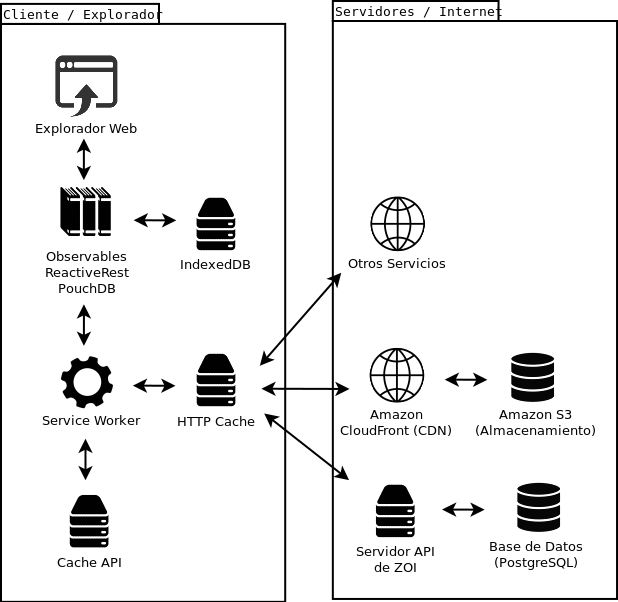
\includegraphics[width=\linewidth]{figures/diagram/diagram.png}
  \caption{Arquitectura Final de la aplicación web de \business}
  \label{fig:diagram}
\end{figure}
